\documentclass[9pt]{pnas-new}
% Use the lineno option to display guide line numbers if required.
% Note that the use of elements such as single-column equations
% may affect the guide line number alignment. 

% \RequirePackage[english,slovene]{babel} % when writing in slovene
\RequirePackage[slovene,english]{babel} % when writing in english
\usepackage{subcaption}

\templatetype{pnasresearcharticle} % Choose template 
% {pnasresearcharticle} = Template for a two-column research article
% {pnasmathematics} = Template for a one-column mathematics article
% {pnasinvited} = Template for a PNAS invited submission

\selectlanguage{english}
% \etal{in sod.} % comment out when writing in english
% \renewcommand{\Authands}{ in } % comment out when writing in english
% \renewcommand{\Authand}{ in } % comment out when writing in english

\newcommand{\set}[1]{\ensuremath{\mathbf{#1}}}
\renewcommand{\vec}[1]{\ensuremath{\mathbf{#1}}}
\newcommand{\uvec}[1]{\ensuremath{\hat{\vec{#1}}}}
\newcommand{\const}[1]{{\ensuremath{\kappa_\mathrm{#1}}}} 

\newcommand{\num}[1]{#1}

\graphicspath{{./figures/}}

\title{Simulation-driven gym layout optimisation}

% Use letters for affiliations, numbers to show equal authorship (if applicable) and to indicate the corresponding author
\author{Andrej Jočić}
\author{Matic Stare}
\author{Martin Starič} 

\affil{Collective behaviour course research seminar report} 

% Please give the surname of the lead author for the running footer
\leadauthor{Jočić} 

\selectlanguage{english}

% Please add here a significance statement to explain the relevance of your work
\significancestatement{Significance statement}{
    A common occurrence in gyms during peak hours is over-crowding of popular equipment and lots of wandering around searching for a free machine.
Through simulating gym-goer behavior, we aimed to identify the most effective arrangement of exercise equipment to improve the flow, accessibility, and overall customer satisfaction.
Our goal is to offer practical insights for gym owners, managers, and designers seeking to optimise their facility layout for the benefit of their clients and business success.
}

\selectlanguage{english}

% Please include corresponding author, author contribution and author declaration information
%\authorcontributions{Please provide details of author contributions here.}
%\authordeclaration{Please declare any conflict of interest here.}
%\equalauthors{\textsuperscript{1}A.O.(Author One) and A.T. (Author Two) contributed equally to this work (remove if not applicable).}
%\correspondingauthor{\textsuperscript{2}To whom correspondence should be addressed. E-mail: author.two\@email.com}

% Keywords are not mandatory, but authors are strongly encouraged to provide them. If provided, please include two to five keywords, separated by the pipe symbol, e.g:
\keywords{gym layout | crowd simulation | gym-goer behaviour | gym traffic}
\begin{abstract}
This report describes our work on simulation-driven gym layout optimisation. We begin with a brief overview of the problem, followed by a description of our agent-based model of gym-goer behaviour. Next, we describe a constrained multi-objective optimisation procedure for finding optimal gym layouts with genetic algorithms, and present some preliminary results. We conclude with a discussion of our solution's limitations and possible future work.
\end{abstract}

\dates{\textbf{\today}}
\program{BM-RI}
\vol{2023/24}
\no{CB:G1} % group ID
%\fraca{FRIteza/201516.130}

\begin{document}

% Optional adjustment to line up main text (after abstract) of first page with line numbers, when using both lineno and twocolumn options.
% You should only change this length when you've finalised the article contents.
\verticaladjustment{-2pt}

\maketitle
\thispagestyle{firststyle}
\ifthenelse{\boolean{shortarticle}}{\ifthenelse{\boolean{singlecolumn}}{\abscontentformatted}{\abscontent}}{}

% If your first paragraph (i.e. with the \dropcap) contains a list environment (quote, quotation, theorem, definition, enumerate, itemize...), the line after the list may have some extra indentation. If this is the case, add \parshape=0 to the end of the list environment.
\section*{Introduction}
% \dropcap{I}
In this report we describe our work on gym layout optimisation.
A common occurrence in gyms during peak hours is over-crowding of popular equipment and lots of wandering around searching for a free machine.
Through simulating gym-goer behavior, we aimed to identify the most effective arrangement of exercise equipment to improve the flow, accessibility, and overall customer satisfaction.
Our goal is to offer practical insights for gym owners, managers, and designers seeking to optimise their facility layout for the benefit of their clients and business success.

To simplify the problem
we will limit ourselves to simulating the behaviour of bodybuilders (performing resistance exercises for muscle hypertrophy).
In this case, a typical workout routine partitions the body into several sets of muscles, cycling through them on a per-workout basis.
%This rotation can be done on a weekly schedule, or the workouts can be weekday-independent for greater flexibility. Popular splits include:
To further simplify the problem, we will only simulate the
\textit{push-pull-legs} (PPL) partitioning\footnote{
    A {\it push} workout consists of pushing movements, mainly targeting the
    chest, frontal deltoids (shoulders), and triceps. Pull muscles are those involved in pulling movements, such as the back musculature, rear deltoids, and biceps. The content of a leg workout is self-evident.
}, which is a popular choice for beginners and intermediate lifters.
We will model the gym as a rectangular grid of cells with pre-set equipment locations, distributed similarly as isles in a grocery store.
% \end{itemize}


\subsection*{Related work}
The only publication related to gym layout optimisation we could find was ref. \cite{turcine2022gym}, which assumed all gym clients had fixed-order workout routines (including ones with weight loss as a goal) and optimised a circular gym layout to minimise backward movement. Unfortunately, this does not give a good foundation for our work, as the assumptions diverge too far from what we are trying to model.

Thus we started from a crowd modelling review \cite{yang2020crowd_modelling_review} for basic model design principles. We also found two articles on incremental urban layout optimisation \cite{feng2016crowd_drive_layout_design, mathew2019urban_walkability} useful when designing the optimisation procedure, especially the cost function.

\section*{Methods}

We used Python's {\it Mesa} library for simulation, analysis, and visualization of agent-based models.

\subsection*{Gym layout model}

\begin{figure}[h]
	\centering
	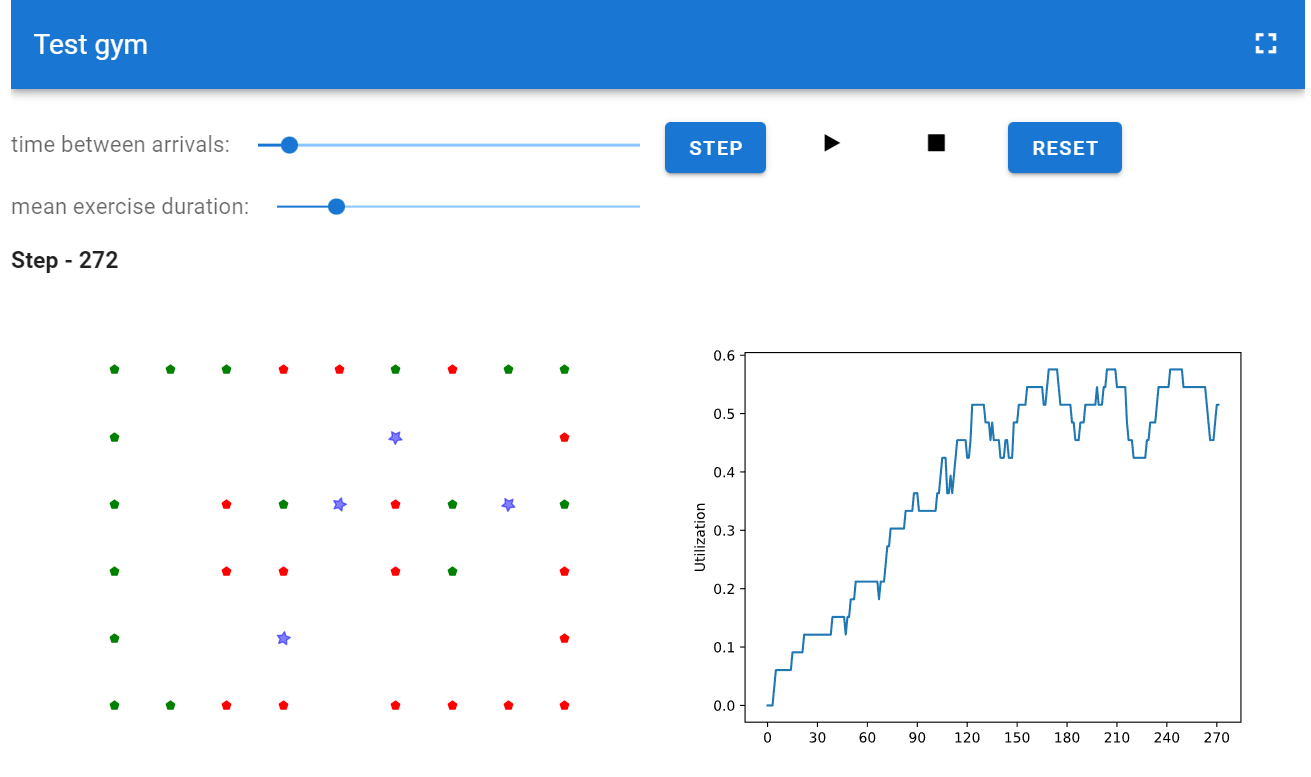
\includegraphics[width=0.8\textwidth]{frozen_simulation_tpl.png}
	\caption{A gym traffic simulation cycle frozen at 272 time steps. On the left we can see the gym environment, generated from a layout template with the entrance at the bottom. Red pentagons are occupied machines, while green ones are free. Agents that are currently walking around in search of a machine are shown with blue stars. On the right, we can see the time progression of one of our gym evaluation metrics (described in a later section).}
    \label{fig:simulation_interface}
\end{figure}


A gym is represented as a subclass of \texttt{mesa.Model} with two rectangular cell grids: the agent layer (where gym-goers move around) and the equipment layer (where machines are statically placed for one simulation cycle).
One cell on the grid's border serves as the locker area entrance, where agents enter the gym.
The agents can only move around in cells that are not occupied by a piece of equipment, but there can be multiple agents in a single cell. We do not feel that agent collision resolution is necessary for realistic modelling of gym traffic. 

For generating a concrete placement of machines, we have to assign certain cells to be equipment locations (where one machine is placed) while making sure we don't create unreachable areas. We have developed some basic layout templates mimicking the arrangement of isles in a grocery store, with sensible walkways in between. In this case, layout optimisation comes down to choosing the best assignment of machines to equipment locations.

\subsection*{Gym-goer behaviour model}

A gym-goer is represented as a subclass of \texttt{mesa.Agent} with a training checklist (multiset of muscles) and its current state.
The agent's goal is to exhaust the checklist as quickly as possible and exit the gym.

A simulation cycle begins with an empty gym. Then, one agent is spawned at the entrance every $t_i$ time steps,
where $t_i$ is a fixed inter-arrival time given as a parameter to the simulation.
When an agent is created, it is assigned a workout routine (e.g. push) and a corresponding workout plan (e.g. chest, chest, triceps, frontal deltoids).
In our experiments we sampled the routine selection from a uniform probability distribution.
The workout plans are constructed ad hoc, in keeping with general workout programming practice.
The agent also keeps track of the machines it has already used, so it can avoid using the same machine twice in one workout.

Upon entering the gym, an agent starts in state {\it searching}, where it looks for a free piece of equipment it can use to check any muscle off its training checklist. A path to the nearest free machine is found using the A* algorithm, which the agent begins to follow.
If the target machine is no longer free upon arrival, the agent continues in state {\it searching}.
When a free machine is found, the agent enters state {\it exercising} and occupies the machine for a certain amount of time. In our experiments, we used a deterministic exercise duration of 30 time steps for all exercises.
After the time has elapsed, the agent re-enters state {\it searching} or exits the gym if it has completed its workout.


\subsection*{Layout optimisation}

We formalized our problem as a constrained multi-objective optimisation problem,
where a layout is constrained by a given layout template.
This constraint makes the optimisation problem more tractable,
and we can also ensure that no unreachable areas are ever created.
With multiple optimisation objectives, we didn't have to combine all aspects of a well-designed gym into one number and thus make arbitrary decisions about the relative importance of each aspect.

The procedure begins with a set of random layouts (meaning random assignments of machines to locations in the template),
and evolves them with a genetic algorithm.
We used Python's {\it PyGAD} library for genetic algorithms, since it supports multi-objective optimisation with the NSGA-II algorithm \cite{nsga2}. This converges to a set of Pareto-optimal solutions, meaning that no other solution can improve on any of the objectives without worsening at least one of the others.

A chromosome in our genetic algorithm is a list of exercise machines. To evaluate a chromosome, we first sequentially assign machines to locations in the layout template.
The locations are ordered in a way that largely preserves the spatial structure of the template,
so that a $k$-point crossover operation doesn't completely destroy the layout topology.
For example, the 4-isle layout template (Figure \ref{fig:2x2_layout}) is ordered as follows: first come the locations around the walls in counter-clockwise order, starting from the bottom-left. Then, all the isles are traversed in row-major order.

After a gym is instantiated, its fitness values are calculated
by running a simulation cycle on it and extracting selected metrics (described in the next section). These metrics constitute the compound objective function.
Note that random mutations and crossover can easily lead to layouts on which some of our hand-crafted workout routines cannot be completed;
we simply set their fitness to negative infinity, effectively discarding them from the population.
In this way, roughly 15\% of solutions were discarded from each generation on average.

We used population sizes around 50 in our experiments. Since this optimisation problem has a complex fitness landscape, we would ideally use even larger ones, but we were limited by the performance of our simulation.
We used a relatively small inter-arrival time $t_i = 2$ to speed up the convergence of optimisation objectives, stopping each simulation after 300 steps.
The random mutation rate was set to 15\%, and we selected the 2-point crossover operator.


\subsubsection*{Objective functions} \label{sec:objectives}

The layout quality metrics which we maximized were: 
\begin{itemize}
	\item agent {\it efficiency}: proportion of time spent exercising, averaged over all agents in the simulation cycle,
	\item gym {\it utilization}: proportion of machines in use at any given time, averaged over the whole cycle, and
	\item gym {\it crowdedness}: proportion of pairs of agents that are ``too close'' to each other at any given time. This was defined as having an inter-cell manhattan distance $\leq 2$, and computed only on agents in state {\it searching}.
    After being averaged over the simulation cycle, this value also had to be inverted since PyGAD only supports fitness maximization.
\end{itemize}



\section*{Results}

We tested our optimiser on a few small layout templates. First we used a template which has machines around the walls and two 2-by-2 islands of machines in the middle (Figure \ref{fig:layout_1}). The fitness functions converged at around 40 generations.
Note that the utilization criterion (\ref{fig:fitness_1}, blue line) decreases as the other two increase. This represents the trade-off between customer satisfaction and gym revenue, as an efficiently utilized gym is cheaper to set up and maintain, but ends up being more crowded.

\begin{figure}[H]
	\begin{subfigure}{0.495\linewidth}
        \centering
        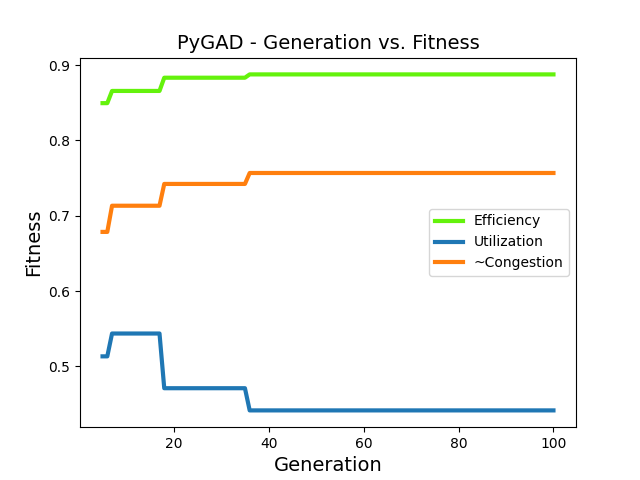
\includegraphics[width=\textwidth]{fitness_1.png}
        \caption{Evolution of fitness functions over generations.}\label{fig:fitness_1}
    \end{subfigure}
    \begin{subfigure}{0.495\linewidth}
        \centering
        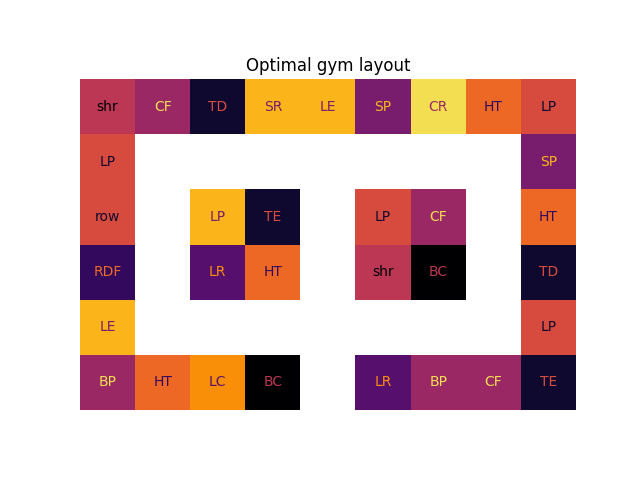
\includegraphics[width=\textwidth]{layout_1.png}
        \caption{A Pareto-optimal gym layout. }\label{fig:layout_1}
    \end{subfigure}
    \caption{Optimisation constrained to a 2-island layout template. Machines (on the right) are labeled with name abbreviations, see the \texttt{Equipment} class in \texttt{gym\_model.py} on our GitHub repository \cite{gymulator} for the list of machines we used. See Figure \ref{fig:colormap} for an interpretation of the colors.}\label{fig:firstTest}
\end{figure}

\begin{figure}[h]
	\centering
	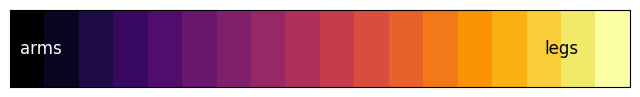
\includegraphics[width=0.6\textwidth]{workoutTypeColormap.png}
	\caption{The colormap we used for visualizing a gym layout. Each machine is colored by the muscle it trains, where muscles are mapped onto the color spectrum in (roughly) the same order as they appear in the human body (from fingertips to heels).}\label{fig:colormap}
\end{figure}

Next, we ran the optimiser on a template with 4 islands of machines (Figure \ref{fig:2x2_layout}). Using the same parameters as before, the optimiser converged after around 110 generations. Due to increasing gym size and a more complex search space, the performance of our simulation prevented us from experimenting with larger layouts.

\begin{figure}[H]
	\begin{subfigure}{0.495\linewidth}
        \centering
        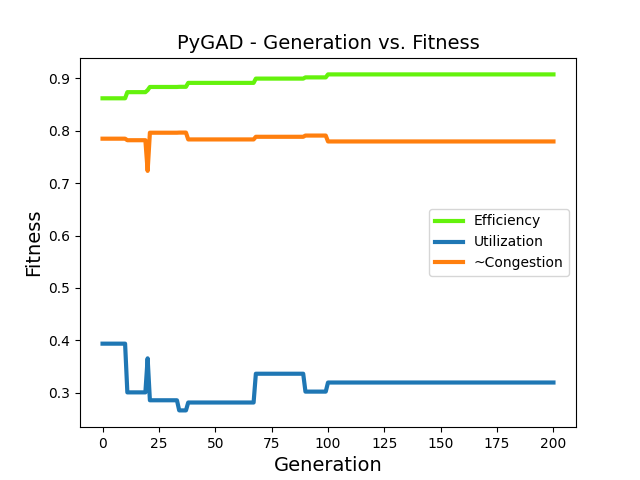
\includegraphics[width=\textwidth]{2x2fitness.png}
        \caption{Evolution of fitness functions over generations.}\label{fig:2x2fitness}
    \end{subfigure}
    \begin{subfigure}{0.495\linewidth}
        \centering
        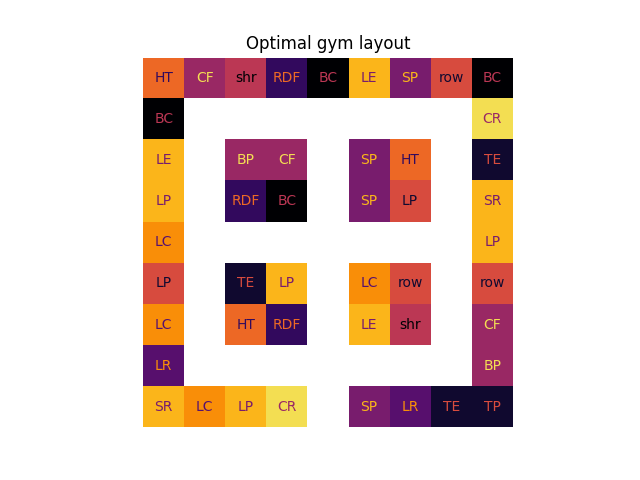
\includegraphics[width=\textwidth]{2x2_layout.png}
        \caption{A Pareto-optimal gym layout.}\label{fig:2x2_layout}
    \end{subfigure}
    \caption{Optimisation constrained to a 4-island layout template.}\label{fig:secondTest}
\end{figure}



\section*{Discussion}

We successfully implemented a gym layout optimisation framework, but our results stand only as a proof of concept.
We made many simplifying assumptions which likely render our model too unrealistic to be of practical use.
Since we didn't invest much time into code optimisation, we couldn't perform comprehensive experiments.
 
\subsection*{Future work} 

Our gym layout model could be made more realistic by dropping the constraints on layout topology and adding support for shared resources (e.g. free weights) and multipurpose equipment.
We could also implement more fine-grained agent behaviour, such as parallel use of gym equipment (where one agent is working while the other is resting), random inter-arrival times (e.g. according to a Poisson process) and random exercise durations,
as well as more realistic routine selection (perhaps with parameters estimated from real-world data).

It would be interesting to let our optimiser come up with a layout from scratch, without the need for hand-crafted templates.
Perhaps this could be done with a Metropolis-Hastings state search variation, which has been successfully applied to urban layout optimisation \cite{feng2016crowd_drive_layout_design,mathew2019urban_walkability}.
Another interesting idea in ref. \cite{feng2016crowd_drive_layout_design} is the use of nonlinear regressors to predict the quality of a layout based on topological features, circumventing the need for computationally expensive simulations.
We could also try to account for the cost of equipment (given by a gym designer) in the optimisation criteria.


\acknow{Everyone worked on the report and gym-goer behaviour model. Andrej Jočić worked on model implementation and the layout optimiser. Martin Starič implemented the pathfinding algorithm. Matic Stare made the project presentation.}

\showacknow % Display the acknowledgments section

% \pnasbreak splits and balances the columns before the references.
% If you see unexpected formatting errors, try commenting out this line
% as it can run into problems with floats and footnotes on the final page.
%\pnasbreak

\begin{multicols}{2}
\section*{\bibname}
% Bibliography
\bibliography{./bib/bibliography}
\end{multicols}

\end{document}